\chapter{Detection Algorithm}
This work focuses on the problem that a compromised switch will bring and presents the method to detect such a switch. Our method emphasizes on scanning though the whole network with fewer packets and high detection efficiency. In this chapter, we will define the threat model and how the problem can be solved with the presented detection algorithm.

\section{Threat models and Attack scenario}
In this work, we assume the following scenario of compromising a switch in the threat model:
\begin{enumerate}
\item
Only one OpenFlow switch is compromised. No cooperation among multiple compromised switches for attacks will happen. 
\item
The switches are able to access the Internet. 
\item
Other parts of the network such as the controller, other switches and hosts function normally. Any potential flaw is unintentional and out of the scope of this work.
\item
An attacker cannot totally change the way of switch processing or core mechanism, but only perform the attack by modifying flow entries.
\item
Initially, the network is clean, and nothing is compromised. The attacks take place some time after the whole network is established.
\end{enumerate}

Other attack scenarios beyond the assumptions such as multiple compromised switches, as well as possible circumvention, will be discussed in Section~\ref{Further_discussion}.

\section{Rapid detection method of disobedient forwarding}
Our method aims to detect if the flow entries of a switch work as expected. It is inspired by \cite{CKGL15}. The method in this work has two main enhancements. First, it reduces the number of detection packets required, and therefore increases the efficiency significantly. Second, no existing flow entry is modified. Only some temporary entries will be added and will timeout after the detection process is over, which has little influence to the whole network and is easy to clean up. 

\subsection{Terminology}

\begin{description}%[font={\small}]

\item
[Aggregation conditions]:
The conditions for an entry to be in the same aggregated group. They can ensure a valid detection packet can be forged and sent through the switches in the group successfully. The conditions are as follows.
\begin{enumerate}[label={\arabic*)}]
\item
In the same group, the flow entries on different switches either have exactly the same match fields and values, or have no common match fields.
\item
A detection packet should not visit a switch more than once.
\item
For a flow entry \textit{A} on a switch, if there exists another flow entry \textit{B} on another switch such that \textit{A} and \textit{B} have the same match field and value, then \textit{A} may belong to more than one aggregated group. Otherwise, \textit{A} \sout{\red{what entries?}} belongs to one aggregated group \sout{\red{what aggregated group? The same as that of A?}}.

\end{enumerate}

\item
[Aggregated groups]: 
A set of entries that satisfy the aggregation conditions. An entry in the group has a forwarding action either to the switch that the next entry \sout{\red{What is the other entry? The other implies only two entries in the group?}} is on or a host. Each group has an integer number as an identifier for detection packets to corespond to.

\item 
[Aggregation tree]
A data structure in a tree format, representing the packet traversal path of an aggregated group. It treats the switches that the entries of the aggregated group are on as vertices, and the forwarding action of those entries as edges. It contains (1) starting switch: the switch as a starting point for traversal, (2) splitting switches: the switches which have more than one child, and (3) leaf switches: the switches which are the leaves of the aggregation tree.

\item
[Detection packets]:
It is forged according to the match fields of the flow entries in an aggregated group. The vid field of each detection packet is set to the group identifier it is associated with.

\item 
[Auxiliary entry]:
The entry that will be added to splitting switches to duplicate the detection packet and send to several \sout{\red{children?}} switches the next entries of the aggregated group are on, or leaf switches to send the packet back to the controller. The match field is selected from a field of the detection packet in order for it to match, in our implementation, the VLAN identifier (vid), which is also the group id of the aggregated group it corresponds to, is selected field as the match field of auxiliary entries. \sout{\red{used for what?}}.
\end{description}

The setups will be explained further in next subsection.

\subsection{The detection method}
\label{Detection_method}

The main idea of the method is to assemble a packet that will go through a sequence of switches by matching the match fields in the flow entries of these switches. Then the packet will be sent into the network, go through the switches, and should be sent back to the controller from expected switches finally if nothing goes wrong. Therefore, the detection packet can check whether the matched flow entries on these switches work as expected or not. For this purpose, we need to find the path that a detection packet should traverse, find the flow entry on each switch with which the packet will be matched, and set the fields in the packet so that it will pass through the switches in order. Because the controller has the network-wise visibility and the policy of all the flow entries, it is able to decide the switches to be involved in an aggregation tree and the detection packet in each run of detection. 

\begin{figure}[H]
\begin{center} 
\includegraphics[width=1\textwidth]{figures/flow_entry_detection_flowchart.png}
\end{center}
\caption{The flow chart of the flow entry detection process.}
\label{flow_entry_detection_flowchart}
\end{figure}

The first aggregation condition is the essential idea of the method: aggregating flow entries this way allows us to forge a packet with multiple fields that match the entries inside the same aggregated group. The second condition is to ensure the detection packet does not get stuck in a loop and never comes back to the controller. The third aggregation condition is also for eliminating loops, we will talk more about it in Section~\ref{Aggregated_group_finding}.

A detection packet is needed for each aggregated group. In other words, minimizing the number of aggregated groups means minimizing the number of detection packets needed, resulting in fast detection. For this purpose, we try to increase the number of entries that one detection packet goes through. On a switch, there may be a collection of entries $E$ that suit the aggregation conditions. We can add a new flow entry with multiple forwarding actions. It will duplicate the detection packet and forward them according to the action set. Therefore, the switches on which the entries in an aggregated group are and their forwarding actions will form a tree. More detail will be stated in Section~\ref{Aggregated_group_finding}.

As the abstraction of the problem, we treat switches as vertices and forwarding from one switch to the next as edges. Our goal is to find the minimum number aggregated groups such that all the entries belong to at least an aggregated group. It forms a complex DAG set covering problem, \sout{\red{note: DAG is a graph, not a problem.}} and is more complex than the longest path problem \cite{DMR97,RU04}, which is NP-complete. Starting from an arbitrary switch, we use DFS to traverse and compose aggregated groups one by one until all the entries belong to at least one group. It can be done in a reasonable amount of time, which will be listed in Section~\ref{Implementation_and_Evaluation}, under the scale of experimental environments.


\subsection{Finding aggregate groups}
\label{Aggregated_group_finding}

The flow chart of the flow entry detection process in the controller is shown in Figure~\ref{flow_entry_detection_flowchart}. Let $S=\{s_1,s_2,\ldots,s_n\}$ be the set of switches under the control of a controller, and $f(s_i)$, where $i=1,\ldots,n$, represents the flow entries on $s_i$. Let $F=\cup_{i=1}^n f(s_i)$, i.e., the set of all the flow entries. In the first step of the flow chart, we attempt to find $A=\{a_1, a_2, \ldots, a_m\}$, the set of aggregated groups, which are set cover of $F$, such that for all the entries in $a_i$, where $i=1,\ldots,m$, satisfy the aggregation conditions.

When finding an aggregated group $a_x$, the $a_x$ is initially empty, and its corresponding detection packet contains no field and value, which is also empty. We start from an arbitrary switch as the starting switch and perform DFS search. While we are at a node of recursion, looking into a switch $s_y$ \sout{\red{Is $s_y$ the starting switch, or what's its relation with the starting switch?}}, we first check if there is any entry which has the match field and value that the detection packet will match \sout{\red{What are the field values in the detection packet in the beginning?}}. If so, the entry is selected and added to $a_x$, not matter it has been in another group or not, as long as the detection packet will match. An undesirable loop may occur at low probability, and we will discuss this situation in the second paragraph of Section~\ref{Further_discussion}. For now, let's assume that no such situation exists. If there are more than one such entry, the one with the highest priority will be selected. If no such entry exists, we search $s_y$ for the entry $E$ which meets the aggregation conditions. That is, the forwarding destination of $E$ has not been visited this round and $E$ belongs to this group only. To see if $E$ belongs to this group only, $E$ should not be used. Also, the switches that the entries are already in $a_x$ are on should not
contain any entry that has the same field and value as $E$, \sout{\red{This sentence is too long and confusing. Break it into a few shorter sentences, or illustrate this case using a figure.}}
otherwise the detection packet will match it first and sent accodingly to its forwarding action, instead of the forwarding action of $E$ as we plan. This corresponds to the third aggregation condition. Once an $E$ is found, it is added into $a_x$. Otherwise, if we cannot find any $E$, $s_y$ becomes a leaf switch, and we return to the parent node of $s_y$ in the aggregation tree and continue to find another $E$. If there is another entry that fits the requirement of $E$, resulting than more than one $E$ in this depth and making this switch a splitting switch, we need to add an auxiliary entry that forwards the detection packet to all the destinations of all the entries that satisfy the condition of $E$. The pseudocode \ref{pseudo} and figure in Figure~\ref{aggregated_group} include this process.

\sout{\red{Again, I suggest to illustrate the case with a figure, so that the reader does not have to imagine the complex case in mind.}}

Regardless of how the selected entry is chosen, the selected entry forwards to a destination, which may be a switch or a host. If the destination is a host, the $s_y$ is also a leaf switch, but in this case we need to install an auxiliary entry on $s_y$ which use \texttt{Packet\_In} to send the detection packet back to the controller. If it is a switch, we move on to the next depth, treating this switch as $s_y$ and start the above procedure all over again until that all layers of fields in the detection packet are taken \sout{\red{What do you mean by ``has no more field available''?}}, or all of the flow entries belong to certain group, and the group finding process for $a_x$ is complete.

The pseudo-code of finding an aggregated group and generating a detection packet is as follows:

\begin {tcolorbox}[blanker,float=tbp,
grow to left by=1cm, grow to right by=1cm]
\label{pseudo}
\begin{algorithm}[H]

  \caption{Packet generating process.}
  \begin{algorithmic}[1]
    \Require
      $switches$: set of switches;  \newline
      $switch$: each switch is a set of entries;  \newline
      $entry$: info of an entry, including match field, value and destination switch;  \newline
      $visited\_switch$: A set of visited switch in one group finding process, cleared every round;  \newline
      $visited\_entry$: A set of visited entries \sout{\red{singular or plural?}} in the group finding processes, and it uses cookies as entry identifiers; \newline
      $packet$: an under-constructing packet that is initially empty and sent after one round of group finding is done; \newline
      $packet[field]$: denotes the value of $field$ in $packet$; \newline
      $aggregated group$: Contains a set of $entry$ in an aggregated group; \newline

      
    \Function{find\_aggregated\_groups}{$switches$}
      \State $\textit{group\_id} \gets 0$;
      \While{\textit{not all the entries have been visited}}
            \State $\textit{starting\_switch} \gets An\;arbitrary\;switch\;with\;unvisited\;entry\;from\textit{switches}$;
            \State $\textit{packet} \gets empty$;   // Cleared per-group finding round \sout{\red{dictionary is undefined.}}
            \State $\textit{aggregated\_group} \gets empty$;
            \State $packet[vid] \gets \textit{group\_id}$;   // Use vid as the group identifier 
            \State $group\_id \gets \textit{group\_id} + 1$;
            \State $\textit{packet} \gets \Call{find\_one\_group}{\textit{starting\_switch}, \textit{packet}, $visited\_switch, $visited\_entry}$;
            \State $Send\;\textit{packet}\;with\;PACKET\_OUT$;
      \EndWhile
    \EndFunction
  \algstore{find_group}
  \end{algorithmic}
\end{algorithm}
\end{tcolorbox}

\begin {tcolorbox}[blanker,float=tbp,
grow to left by=1cm, grow to right by=1cm]
\begin{algorithm}[H]
  \begin{algorithmic}[1]
  \algrestore{find_group}
    \Function{find\_one\_group}{switch$, packet$, $visited\_switch$, $visited\_entry$}
      \If{$switch < 0$} //it's a host
        \State \Return $packet$;
      \EndIf
      \State Add $switch$ to $visited\_switch$;
      \State $\textit max\_priority \gets -1$;  
      \ForAll{$entry\;in\;switch$}
        \State $\textit{field, value, priority} \gets extract(\textit{entry})$;
        \If{ $packet[$field$] is defined \textrm{ and } packet[$field$] == value \textrm{ and } priority > max\_priority$} //get the one with highest priority 
          \State $\textit{max\_priority} \gets \textit{priority}$;
          \State $\textit{selected\_entry} \gets \textit{entry}$; 
        \EndIf
      \EndFor

      \If{$max\_priority \neq -1$} //found an entry that the packet matches
        \State Add the cookie of $selected\_entry$ to $visited\_entry$;
        \State $\textit{destination} \gets extract(\textit{entry})$;
        \If{$destination$ is a host}
          \State Add auxiliary entry that forward back to the controller;
          \State \Return $packet$;
        \Else
          \State Add $entry$ to $aggregated\_group$;
          \State \Call{find\_one\_group}{$destination$, $packet$, $visited\_switch$, $visited\_entry$}; //move on to next depth
        \EndIf
      \EndIf
  \algstore{find_group}
  \end{algorithmic}
\end{algorithm}
\end{tcolorbox}

\begin {tcolorbox}[blanker,float=tbp,
grow to left by=1cm, grow to right by=1cm]
\begin{algorithm}[H]
  \begin{algorithmic}[1]
  \algrestore{find_group}
      \State // no entry in this switch has match field and value already in packet;
      \State $\textit{output\_set} \gets empty$;  //  the output ports auxiliary entry out to
      \State $\textit{entry\_fit} \gets empty$; 
      \ForAll{$entry\;in\;switch$}
        \State $\textit{field, value, destination, cookie} \gets extract(\textit{entry})$;
        \If{$cookie$ not in $visited\_entry$ and $destination$ not in $visited\_switch$ and no entry with same field and value exist in $parent\_switch$ for all $\textit{parent\_switch} \in \textit{visited\_switch}$} 
          //  entry that fit aggregation conditions
          \State Add $entry$ to $aggregated\_group$;
          \State $\textit{packet}[\textit{field}] \gets \textit{value}$;  //add match field to detection packet
          \State Add cookie of $selected\_entry$ to $visited\_entry$;
          \State Add output port to destination to $output\_set$
          \If{$destination$ is a host}
            \State Add auxiliary entry on $switch$ with forwarding action back to the controller;
          \EndIf
          \State \Call{find\_one\_group}{$destination$, $packet$, $visited\_switch$, $visited\_entry$}; 
        \EndIf
      \EndFor
      \If{$output\_set$ has more than one element}
        \State $Add\;auxiliary\;entry\;on\;\textit{switch}\;with\;forwarding\;action\;to\;elements\;\in\;
        \textit{output\_set}$;
      \EndIf
      \State \Return $packet$;
    \EndFunction
\end{algorithmic}
\end{algorithm}
\end{tcolorbox}

After finding the aggregated group $a_x$, the controller will send a detection packet with \texttt{PACKET\_OUT} to the starting switch, and the detection packet will pass the through the switches in the aggregation tree \sout{\red{tree or trees?}}. The detection packets should also meet the dependency requirement stated in the third paragraph of Section~\ref{SDN and OpenFlow}; otherwise, it will not be matched by any flow entry. When it arrives at a splitting switch, it will be duplicated and sent to more than one switch due to the auxiliary entry we install on the splitting switch. Eventually, when the detection packet reaches the last entry in $a_x$, it will be sent to a leaf switch which either contains no flow entry in $a_x$ or forwards to a host. In the former case, the packet will fail to match any flow entry on that switch and be sent back to the controller due to the table-miss entry, while in the later case, the leaf switch will send the detection packet back to the controller by the auxiliary entry. 

To analyze the time complexity, let the number of all entries in the network be $E$, average number of entries in each switch be $ES$, average number of entries in each aggregated group be $EG$, and number of aggregated group be $G$. In each depth of find an aggregated group, we need $O(ES)$ for checking if the detection packet matches any of the entry in the packet. After ensuring that no such entry exists on this switch, we need $O(ES * ())$ \red{$\leftarrow$ error} for checking through all the entries on this switch, where $E$ is to check if the entry is used already, the first $EG$ to check if the switch is visited, the second $EG$ to check if the entry fits without any conflict fields, and $EG*ES$ to check if there exists any entry with same field and column exist on switches which the entries already in this group are on. In total, the time spent each depth will be $O(ES) + O(ES* (E+EG+EG+EG*ES) )$, which equals to $O(E*ES + ES^2*EG)$. Thus, the total time complexity of all aggregated groups finding will be $O(E*ES + ES^2*EG) * EG * G$, which equals to $O(E*S*EG*G + ES^2*EG^2*G)$. Since $G$ Packet\_Outs will be sent, the time for \texttt{Packet\_In} checking process is between $O(G)$ and $O(G*EG)$.

Figure~\ref{aggregated_group} illustrates an example with a complete aggregated group with group identifier 1 and its corresponding detection packet. We have a controller, three switches, $s_1$, $s_2$ and $s_3$, and a detection packet. $s_1$ is a starting switch as well as a splitting switch. $s_2$ and $s_3$ are leaf switches \sout{\red{No $s_b$ and $s_c$ are shown in the figure}}. The solid lines are the traveling path of detection packet, the dash lines are \texttt{Packet\_Out} and \texttt{Packet\_In} from and to the controller, and the direction of the arrow is the direction that the detection packet is sent to. The entries colored with green will be matched by the detection packet. Fields of entries other than matched field and value are omitted for simplicity. There are multiple entries on every switch, but only the entries that are in the aggregated group are shown\sout{\red{... wrong grammar}}.

There are three entries on $s_1$: one with match field \texttt{eth\_dst}=\texttt{a2:b4:c6:d8:e0:f1} and an output action to $s_2$, one with match field \texttt{eth\_src}=\texttt{b1:c0:aa:03:51:6b} and an output action to $s_3$, and an auxiliary entry that duplicates the detection packet and sends them to $s_2$ and $s_3$. $s_2$ has an entry with match field \texttt{ipv4\_src}=\texttt{140.123.103.123} and an output action to host, and also an auxiliary entry that sends the detection packet back to the controller. According to the match fields of these flow entries in the aggregated group, the forged detection packet contains \texttt{eth\_src}=\texttt{b1:c0:aa:03:51:6b}, \texttt{eth\_dst}=\texttt{a2:b4:c6:d8:e0:f1}, \texttt{ipv4\_src}=\texttt{140.123.103.123} and \texttt{vid}=\texttt{1}. After the aggregated group with groupd id 1 is found\sout{\red{After what?}}, the controller sends the detection packet to $s_1$ \sout{\red{No $s_a$ is shown in the figure}}, it will be duplicated and sent to $s_2$ and $s_3$. Since the forwarding action of the entry in $s_2$ redirect \sout{\red{direct what?}} to a host, the packet will be sent back to the controller by the auxiliary entry. The packet sent to $s_3$ will be sent back by table-miss. The controller sends one packet out and receives two packets, since there are two leaf switches.

\begin{figure}[H]
\begin{center}
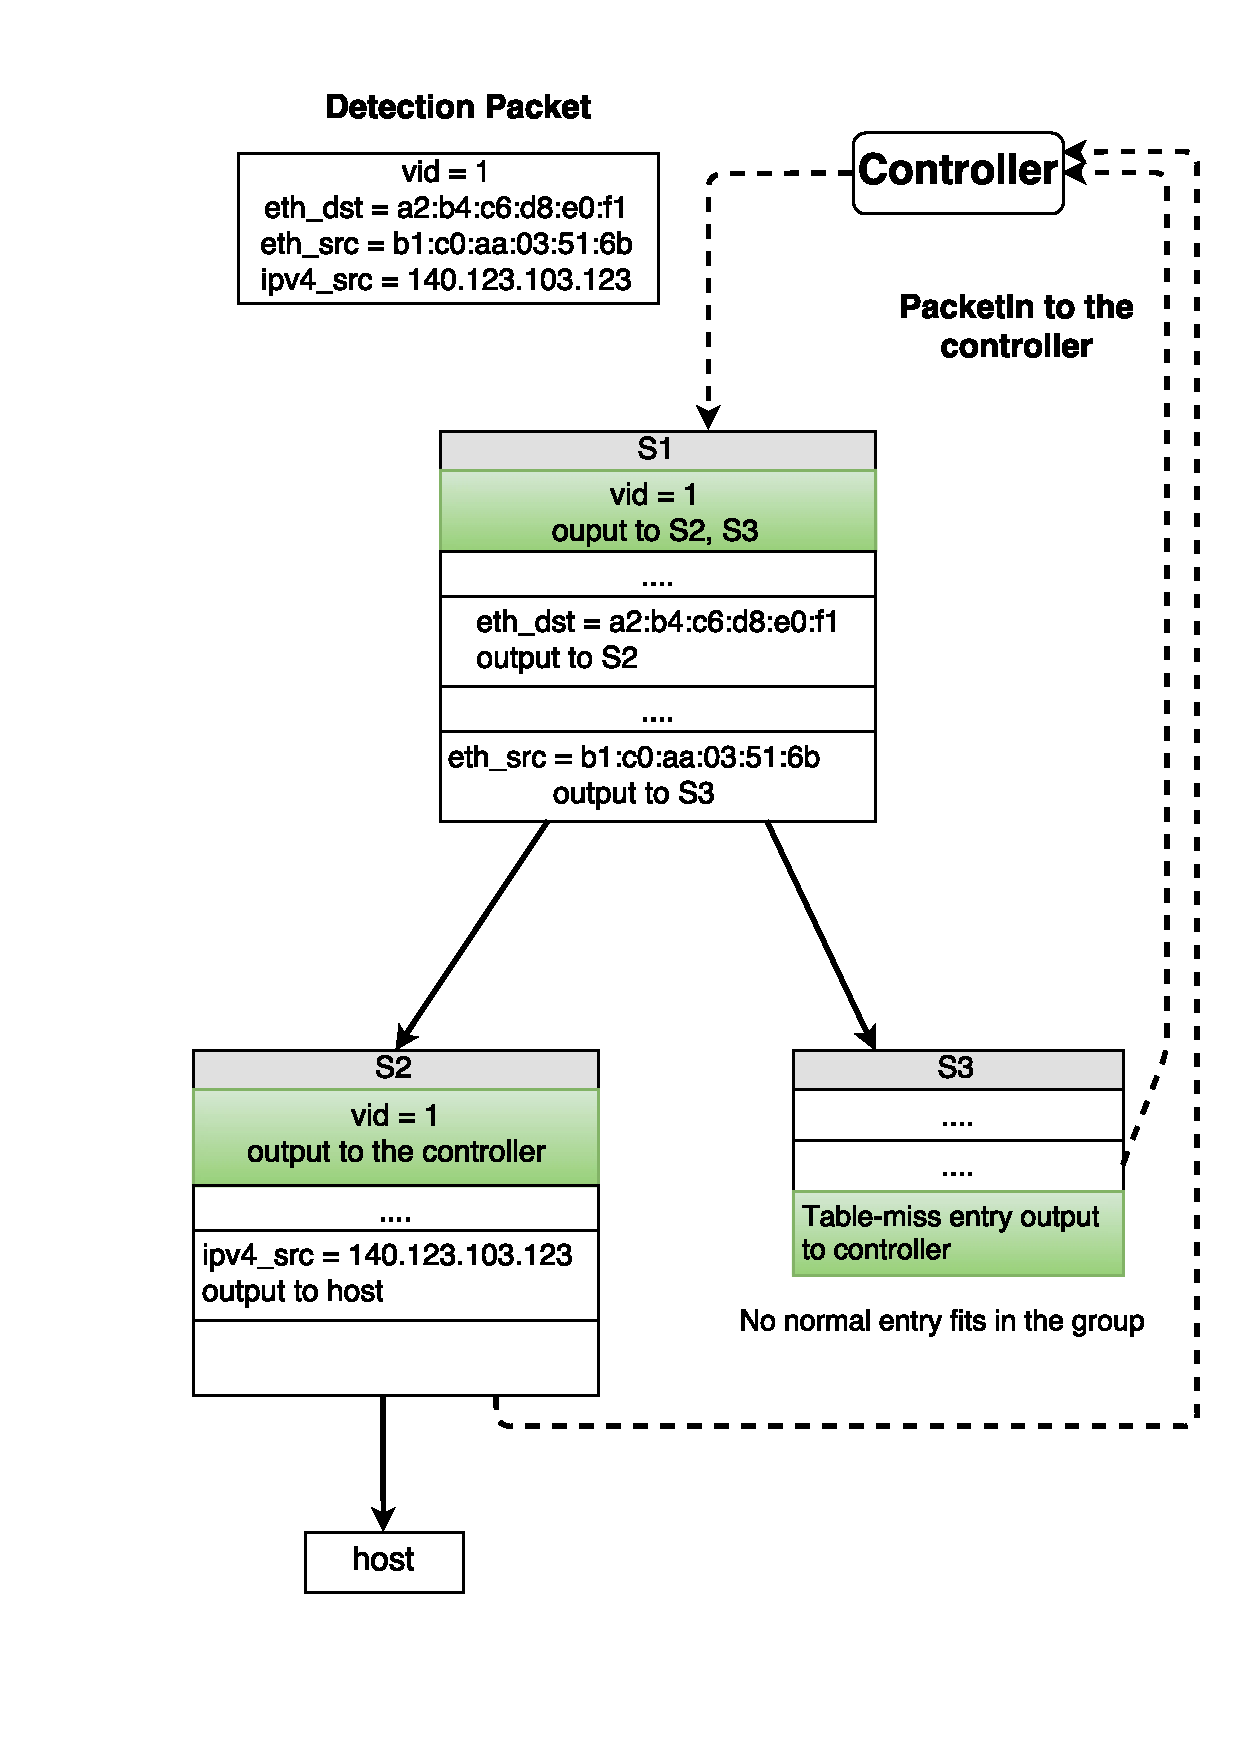
\includegraphics[width=1\textwidth]{figures/aggregated_group.pdf} %XXXXXXXX
\end{center}
\caption{An aggregated group and constructed dectection packet. \sout{\red{wrong figure}}}
\label{aggregated_group}
\end{figure}

\subsection{Checking detection packets on the controller}
The controller checks two things to see if the forwarding actions of all entries work as expected. First, when it receives \texttt{Packet\_In}, it checks the \texttt{vid} field of the detection packet. The packet is expected to come back from one of the leaf switches in the aggregated group the \texttt{vid} is associated with. If the \texttt{vid} is not one of the leaf switches, then the controller should raise an alarm. Second, the controller waits for the detection packets to come back. After the time that all the detection packets should arrive, it checks all the leaf switches, where the \texttt{Packet\_In} is expected to come back from, to see if any switch does not send back a \texttt{Packet\_In} as expected, and raises an alarm if there is any. 

\subsection{Further discussion of attack scenario and our method}
\label{Further_discussion}
On splitting switches and leaf switches, we install auxiliary entries. However, this will make the detection packet match auxiliary entries rather than the original ones. To deal with this problem, the egress processing, newly introduced in OpenFlow 1.5 \cite{OF_SPEC_15} should be used. With egress processing enabled, we are able to add the auxiliary entries in the egress table, which will be processed after the output action and let the original entries match prior to the auxiliary entries, and no entry will be missed. For the OpenFlow version former than 1.5, we should choose a field for the auxiliary entries that does not conflict with the existing entry in the switch on which it is installed with high priority to ensure that the auxiliary entries will be matched prior to other entries.

In the second paragraph of Section~\ref{Aggregated_group_finding}, we mentioned that the entry that may force a loop if it contains the match field and value that the detection packet will match. This happens when it forwards the packet to a parent node in the aggregation tree by chance. In reality, there are mechanisms like spanning tree protocol to deal with the loop problem. However, implementing such a mechanism is external to this method. In our implementation, we simply remove the particular switch from the aggregation tree that causes a loop. This ad-hoc implementation is sufficient for our experiment, and should make the experiment go on as normal.

The trait of match field mentioned in the third paragraph of Section~\ref{SDN and OpenFlow} makes match field aggregation much more complicated. The situations can still be covered by our method with some modification if we manage to resolve the complex conjunctive conditions. Take the entry with multiple match fields for example, if all the fields and values match the under-constructing packet, we process it according to first aggregation rule. Otherwise, we fill the packet with all of those match fields. If any match field has been already taken with a different value, it will be ignored for this turn of aggregation process and fill the match fields in another packet that has no conflict field. For example, if a packet has TCP source port 80 and TCP destination port 123, and it meets an entry with match fields tcp source port 80 and destination port 456, the entry cannot fit into the aggregated group the packet associates to even if the source port matches, since it has a destination port that will not match.\sout{\red{Give an example for this.}} However, the main purpose of our method is to show the effectiveness of flow entry aggregation method. We will demonstrate with the simplest condition, which is that every entry has only one matching field and uses only one flow table.

It is certainly possible that multiple switches are made by the same manufacturer or have common software version in the same network, so multiple switches share common vulnerabilities and may be compromised simultaneously. However, cooperation between multiple compromised switches complicates the scenario significantly. To simplify the case as a starting point for developing the detection method, we assume only one switch inside the network is compromised.

Suppose an attacker is able to add, remove, or modify the entries in the flow tables of a compromised
switch without notifying the controller, so packets may be forwarded to an undesired destination. The proposed method is intended to detect this behavior with high efficiency. In this method, only the output action of packets is considered. Other actions such as dropping packets, setting field and changing TTL are not included. Although there may be reasonable ways to deal with these actions, for example, to detect packet dropping, we can add timeout checking function. Such a detection function is irrelevant to our main method and is not implemented in this work.

In this detection method, there is another important consideration: the controller must maintain unpolluted information of all flow entries. It is not reliable for a controller to obtain flow entry information by querying switches because a switch may be compromised and forge a fake response that gives false information about the flow entries. That is the reason for the last statement of the attack model. Also mind that the detection packet should not be distinguishable from a normal packet; otherwise, the attacker will be able to circumvent the detection method.